\cvsection{Selected Projects}

\begin{cventries}

  \cventry
    {Python · Vue 3 · MCP · RAG}
    {Multi-Agent Shopping Assistant}
    {\href{https://github.com/Sophie618/Multi-Agent}{GitHub}}
    {Nov. 2025 -- Present}
    {
      \begin{cvitems}
        \item {Built an e-commerce assistant around the Model Context Protocol, implementing the LLM $\rightarrow$ Router $\rightarrow$ MCP Server $\rightarrow$ Backend API tool-calling pipeline.}
        \item {Explored a Planner--Worker multi-agent architecture and developed a Vue 3 conversational interface that renders structured tool results as visual product cards.}
      \end{cvitems}
    }

\vspace{0.8cm} % 手动增加条目间距，数值按需调0.2~0.6cm
  \cventry
    {FastAPI · React · LLM · Prompt Engineering}
    {Collector+ (Collector-AI)}
    {\href{https://github.com/Sophie618/Creator_ai}{GitHub} · \href{https://collectorai.top/}{Live Demo}}
    {Jan. 2026}
    {
      \begin{cvitems}
        \item {Built a low-latency information extraction and gamified-reading assistant that transforms long-form articles and videos into binary prediction questions and supports source-grounded Q\&A over saved content.}
        \item {Designed a linear-monolithic asynchronous pipeline with approximately 15--30 seconds of end-to-end generation latency and general-purpose parsing for WeChat articles, Bilibili videos, and dynamically rendered pages.}
        \item {Implemented structured prompt engineering and an intuition-driven interaction flow with React Context state management.}
      \end{cvitems}
    }
    
\vspace{0.8cm} % 手动增加条目间距，数值按需调0.2~0.6cm
  \cventry
    {Next.js 16 · React 19 · DeepSeek-V3 · Zustand}
    {FitSnap}
    {\href{https://fit-snap-beige.vercel.app/}{Live Demo}}
    {Dec. 2025}
    {
      \begin{cvitems}
        \item {Transformed unstructured instructional videos into structured, timestamped steps with action categories and key parameters using schema-constrained JSON output.}
        \item {Built a content-agnostic generative UI with bidirectional synchronization between video playback and task-specific step cards for fitness, cooking, and other instructional content.}
      \end{cvitems}
    }
    
\vspace{0.8cm} % 手动增加条目间距，数值按需调0.2~0.6cm
  \cventry
    {React · D3.js · Three.js · Python}
    {BiGEM Data Retrieval and Visualization Platform}
    {\href{https://gitlab.igem.org/2025/software-tools/bit-china}{Source} · \href{https://2025.igem.wiki/bit-china/software}{Project Wiki}}
    {Sep. 2024 -- Oct. 2025}
    {
      \begin{cvitems}
        \item {Collected, cleaned, and connected iGEM data from 2004--2024 and visualized global collaboration networks using force-directed graphs, trees, and Sankey diagrams.}
        \item {Integrated LLM-based semantic analysis to improve retrieval of biological parts and historical projects; received a 2025 iGEM Gold Medal and Best Software in the undergraduate category.}
      \end{cvitems}
      % Portfolio version only:
      % \begin{center}
      %   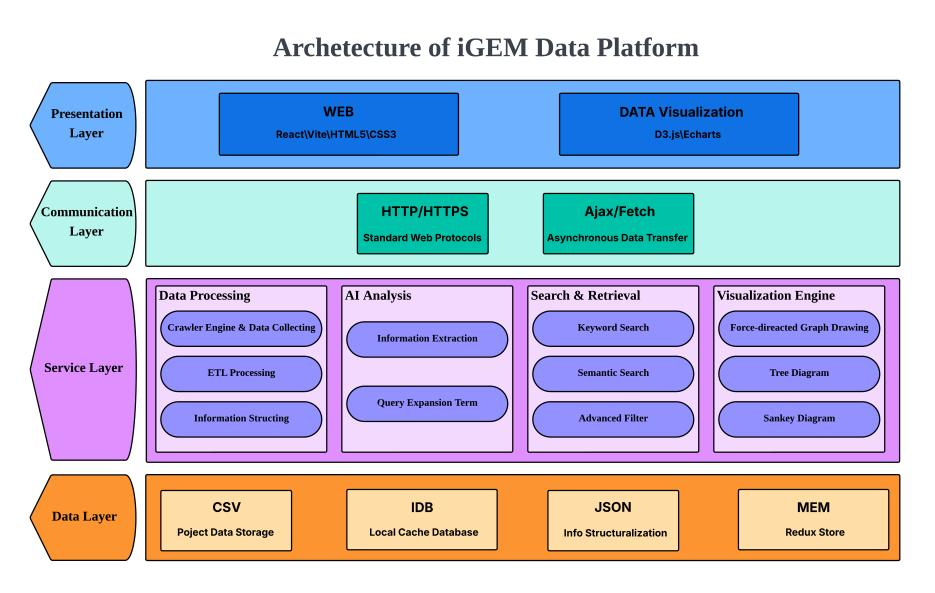
\includegraphics[width=0.82\linewidth]{assets/bigem-architecture.png}
      % \end{center}
    }

\end{cventries}
